% -*- coding: utf-8; -*-

\chapter{Situa{\c c}\~ao Atual}
\label{cha:Situa{\c c}\~ao Atual}

\section{Serviços disponibilizados}

O microhorario\footnote{https://www.puc-rio.br/microhorario} é um serviço disponibilizado pela universidade para consultar informações das disciplinas do semestre atual. Este possui uma interface simples que pode ser visualizada na figura \ref{fig:microhorario}. Essa interface permite filtrar disciplinas por seus atributos como nome, código, professor e departamento. Porém, essa interface não é personalizada com relação ao aluno, ou seja, não exibe as disciplinas que o aluno em específico ainda não cursou ou que o aluno não pode cursar devido à pré-requisitos.

\begin{figure}[h]
    \begin{center}
    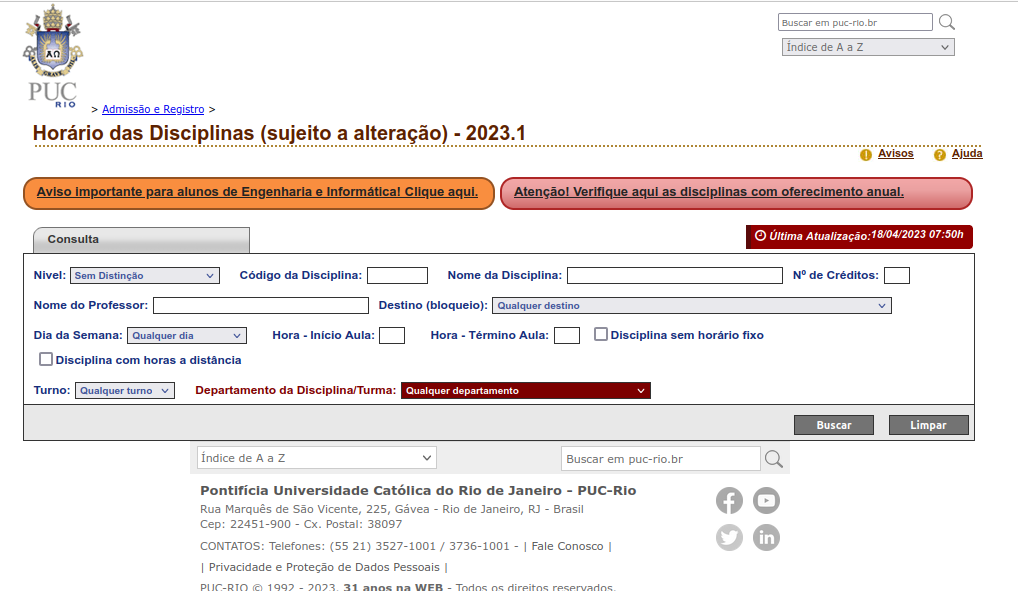
\includegraphics[width=300pt]{figuras/microhorario}
    \caption{Interface do \textit{microhorario}}
    \label{fig:microhorario}
    \end{center}
\end{figure}

Para consultar a grade recomendada e os pré-requisitos, o aluno precisa acessar um documento\footnote{http://www.inf.puc-rio.br/wordpress/wp-content/uploads/2023/01/\\Grade\_Eng\_comp\_2023.pdf} presente na página do departamento ou acessar o currículo disponibilizado na página da universidade. A grade recomendada possui os nomes das disciplinas e seus pré-requisitos, mas não contém a disponibilidade do próximo período.

Além disso, as disciplinas eletivas que o departamento oferece durante o semestre são anunciadas em diferentes veículos de comunicação, como e-mail, página da coordenação do curso, ou folhetos em corredores do departamento. Não há uma distribuição centralizada das ofertas de disciplinas eletivas, portanto o aluno pode não saber aonde procurar essas ofertas, e perder boas oportunidades por desconhecer o anúncio da disciplina eletiva.
\section{Processo de matrícula}

A matrícula na PUC-Rio é um processo que dura vários dias. A universidade divulga o agendamento de matrícula, em que cada aluno recebe uma data e hora para realizar sua matrícula. As datas possíveis abrangem um período de cinco dias. Durante o período de matrícula, o microhorario atualiza periodicamente para indicar quais turmas ainda possuem vagas disponíveis, e se houve o cadastro ou cancelamento de alguma outra disciplina durante este período.

Portanto, é comum que um aluno crie formas de planejamento próprias para conseguir organizar todo o fluxo de dependências, anotar as disciplinas que estão sendo oferecidas, assim como suas turmas e professores. Esses dados precisam estar em constante atualização durante o período de matrícula, conforme as vagas vão sendo preenchidas e a disponibilização de novas turmas ou disciplinas são anunciadas. Este é um processo que maximiza a qualidade da sua grade horária, mas demanda muito esforço e tempo. 

A universidade disponibiliza um simulador de matrícula por um curto período antes do processo de matrícula em si. A interface do simulador é a mesma da matrícula, como pode ser observado na figura \ref{fig:simulador}, 
afim de o aluno poder simular a criação da sua grade de disciplinas para o próximo semestre. O simulador apresenta os dados das disciplinas atualizados conforme o microhorario, e os disponibiliza de três formas diferentes: buscas por disciplinas que faltam cursar no currículo do aluno, buscar por nomes de disciplinas e buscar por horários das turmas das 
disciplinas.\cite{doc-matricula}

\begin{figure}[!ht]
  \begin{center}
  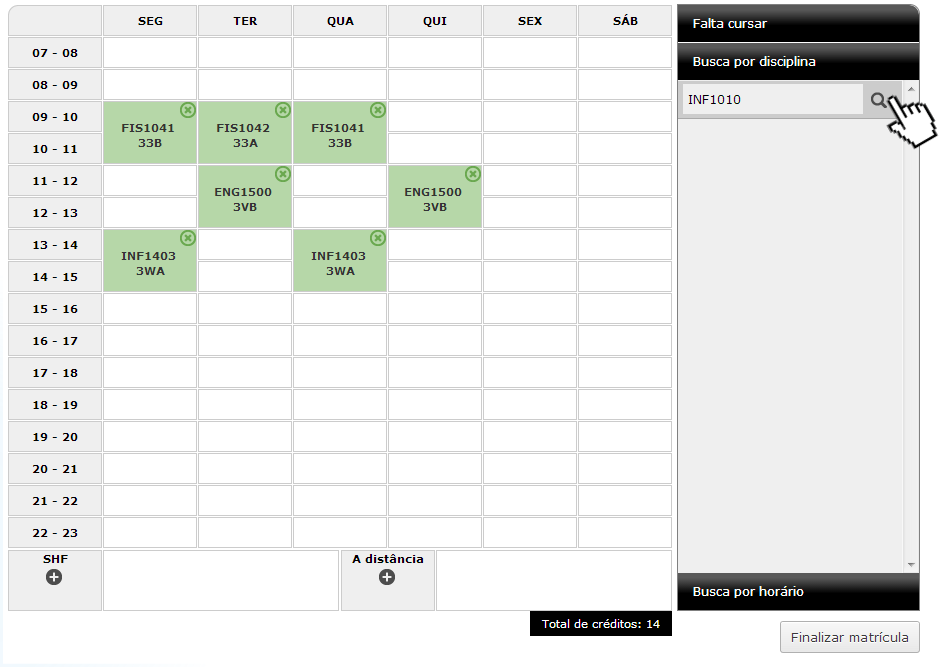
\includegraphics[width=250pt]{figuras/simulador}
  \caption{Interface do simulador}
  \label{fig:simulador}
  \end{center}
\end{figure}

\section{Estudos relacionados}

A escolha de disciplinas é um problema comum em universidades que possuem algum grau de flexibilidade na grade horária. Ng \& Linn\cite{crs-recs} desenvolveram um sistema de recomendação de disciplinas para a sua universidade chamado CrsRecs que utiliza análise de sentimento, pontuações de professores e disciplinas, e preferências que o aluno escolhe fornecer. A vantagem do CrsRecs é não depender de dados privados da universidade como notas e avaliação dos alunos nas disciplinas, utilizando somente informações fornecidas diretamente pelo usuário. Mas há também um esforço na decodificação das informações fornecidas, o que pode ocasionar recomendações incorretas provenientes da má interpretação do usuário.

Há estudos que utilizam históricos escolares dos alunos para gerar modelos de previsão de notas.\cite{rani-machine-learning,nguyen-learning-outcome,adak-fuzzy} Nesse caso, o objetivo do modelo é tentar prever quais disciplinas o aluno tem a maior chance de obter uma boa nota, mas não necessariamente prever quais delas mais combina com o aluno.\cite{rani-machine-learning,nguyen-learning-outcome}

A escolha de disciplinas eletivas também é uma preocupação presente nas universidades. Na PUC-Rio e em outras universidades, os currículos de graduação solicitam créditos de disciplinas eletivas, seja dentro do departamento da graduação do aluno ou não. O sistema do estudo de Adak et al.\cite{adak-fuzzy} recomenda disciplinas dentro de um departamento que parecem se relacionar com o histórico escolar do aluno, mas excluem disciplinas fora do departamento.
Já o sistema de Xu et al.\cite{xu-personalizado} recomenda uma sequência de disciplinas eletivas que maximem a sua nota e não aumentem o tempo de conclusão da graduação do aluno, levando em conta dados históricos do aluno e a disponibilidade atual das disciplinas. 
Por último, o estudo de Adak \& Ercan\cite{adak-svm} utiliza dois algoritmos de inteligência artificial de aprendizado supervisionado, support vector machine (SVM) e árvores de decisão, para recomendar eletivas que mais se assemelham ao aluno, utilizando dados históricos do aluno tanto para o treinamento dos modelos de algoritmo como para a recomendação.

O comum nos estudos é a tentativa de maximizar a nota média do aluno utilizando os dados históricos de alunos da universidade para treinar modelos de inteligência artificial.\cite{rani-machine-learning,nguyen-learning-outcome,adak-fuzzy,adak-svm} Porém, o foco específico nos resultados pode ocultar oportunidades de disciplinas que o aluno poderia se interessar.

% Early smoothing methods tried to minimize... In the figure \ref{subfig:pictures/image01.png} we see...

% \subimages{A set of three subfigures:
% (a) describes the first subfigure;
% (b) describes the second subfigure;
% (c) describes the third subfigure.}{55}
% {
%  \subimage[Bamboo-pile Vertically Inserted Position]{.45}{pictures/image01.png}
%  \subimage[Bamboo-pile Normal Inserted Position]{.45}{pictures/image02.png}\\
%  \subimage[bamboo-pile Inserted 45° angle]{.45}{example-image}
% }
% \newpage
% \csubimages{A set of six subfigures in two pages.}{55}
% {
%  \subimage[Bamboo-pile Vertically Inserted Position]{.45}{pictures/image01.png}
%  \subimage[Bamboo-pile Normal Inserted Position]{.45}{pictures/image02.png}\\
%  \subimage[bamboo-pile Inserted 45° angle]{.45}{example-image}
% }
% \ssubimages{A set of six subfigures in two pages.(Continuation)}{55}
% {
%  \subimage[Bamboo-pile Vertically Inserted Position]{.45}{pictures/image01.png}
%  \subimage[Bamboo-pile Normal Inserted Position]{.45}{pictures/image02.png}\\
%  \subimage[bamboo-pile Inserted 45° angle]{.45}{example-image}
% }